\documentclass[11pt]{article}
\usepackage{amsmath,amssymb,graphicx,booktabs,multirow,url}
\title{Myna: A Measurement Study of Typed Agent Decision Engines}
\author{Aashish Kumar Mahato\\Independent Researcher, Kathmandu, Nepal\\
\small Graduate of Vellore Institute of Technology (VIT), Vellore, India. This work was conducted
independently after graduation.}
\date{November 2026}
\begin{document}
\maketitle
\begin{abstract}
Typed decision engines score a fixed option set instead of generating text. This paper reports a
measurement study of Myna, two engines behind one typed choice/score/noul contract: a 14.45M
gated-linear-attention streaming engine with a 576 KiB state, and a 446.63M fine-tuned
DeBERTa-v3-large with a cardinality-routed readout. On a frozen 16-cell suite (1,176 bundles,
1,440 questions) Myna v6 reaches 0.7777 macro against five external systems: a supervised
TF-IDF classifier (0.7111), three configurations of Laya 0.4.19 (0.7050 best), VegaML 0.15.0
(0.6160), a train-prior majority classifier (0.3726), and a zero-shot NLI scorer (0.3278). The
comparison is in-domain for Myna and out-of-domain or zero-shot for the engines, so it is
reported as a footing-qualified comparison rather than a leaderboard claim. Three results are
negative. Cardinality routing is a budget repair worth 0.0399 macro on exactly one cell, and the
isolated ablation on one checkpoint shows the other 15 cells identical. Cross-question
consistency is an observed property of the encoder, not an enforced constraint (3/172
contradictions against 31/172 and 32/172 for the external engines). Split-conformal sets cover
85.49% at a 90% target and are reported as unusable for abstention; calibration error (ECE
0.0637) and risk-coverage replace them. The audit also exposes that the ordinal primitive is at
chance (0.1750 over 240 five-way questions) while the choice and boolean primitives reach 0.8908
and 0.9385. The revision documents and corrects a scoring error that had inflated the macro from
0.7777 to 0.8620; every figure in this paper is recomputed from released per-question records.
\end{abstract}
\section*{1. Introduction}
An agent that processes tickets, threads, or page states asks many small questions: whether a
message is a refund request, how severe it is, which department owns it. Each question has a
small, fixed answer set, and the state on which it is asked grows with every turn.
Autoregressive language models answer such questions fluently but pay for generation on every
call and can return text outside the option set. A non-autoregressive \emph{decision engine}
instead returns a categorical distribution over predefined options
[1, 2]. The design is attractive for high-frequency routing, but three
properties determine whether it can be deployed: whether the option set fits the model's input
budget, whether the confidence it reports can support abstention, and whether the answers to the
questions of one bundle are mutually consistent.

This paper reports a measurement study of Myna, two engines behind one typed
\texttt{choice}/\texttt{score}/\texttt{noul} contract. Myna-Stream{} is a 14.45M-parameter
gated-linear-attention engine whose retained state is 576 KiB at every length from 128 to
16{,}384 tokens. Myna-v6{} is a 446.63M-parameter fine-tuned DeBERTa-v3-large with a
cardinality-routed readout; it re-encodes the state on every question and is the accuracy arm.
The two share the question schema, the answer record, the abstention seam, and the serving API,
and nothing else. A latency measurement on one engine is therefore not a statement about the
other, and the paper keeps the two apart throughout.

The study is conducted on \textsc{decision-v2-pilot}, a frozen suite of 1{,}176 test bundles and
1{,}440 questions over 16 cells drawn from 11 public sources (Table~1). Every arm
is scored on the same rows, and every aggregate is recomputed from released per-question records
by a single script (\texttt{bench/paper\_numbers.py}), so a table cannot drift from the records
it cites.

\textbf{Contributions.} The paper makes five contributions; two are negative results and a
third is a documented correction.

\begin{itemize}
\item \textbf{A like-for-row comparison with five external systems.} The same 1{,}176 test
bundles are scored by Myna-v6{}, by three configurations of a contemporary decision engine
(Laya 0.4.19), by a second engine (VegaML 0.15.0), and by three classical references: a
train-prior majority classifier, a supervised TF-IDF classifier, and a zero-shot NLI scorer.
Myna-v6{} reaches 0.7777 macro against 0.7111 for TF-IDF, 0.7050 for the best Laya configuration,
0.6160 for VegaML, 0.3726 for the majority classifier, and 0.3278 for NLI. The comparison is
in-domain for Myna-v6{} and out-of-domain or zero-shot for the others, and
Section~5 states that footing with each number.
\item \textbf{A cardinality-budget diagnosis and an isolated routing ablation.} The packed
layout fits every cell with $K\le15$ options. The 77-way cell overflows on 50 of 116 rows,
consumes 490 option-span tokens (6.36 per option), and collapses. Forcing the packed scorer on
every cell, with the weights held fixed, scores 0.0345 on that cell and 0.7378 macro; enabling
the router on the same weights scores 0.6724 and 0.7777. No other cell changes. Routing is a
budget repair for one cell, worth $+0.0399$ macro, and the paper presents it as such.
\item \textbf{Bundle consistency as a measured property, with both predicates released.} The
checkpoint records 0/172 contradictions. That record is reproduced by the campaign's own rule,
recovered from the released notebook (0/172 for Myna-v6{}, 1/172 for Laya, 2/172 for VegaML), but
the rule only inspects choice--boolean pairs and cannot see the yelp rating/recommendation case. A
broader released predicate (\texttt{src/myna/consistency.py}) gives 3/172, 31/172, and 32/172. The
cross-question graph head is never called at inference and its gate is zero in the released
ablation, so consistency is a property of the fine-tuned encoder rather than an enforced
constraint, and no architectural claim is attached to it.
\item \textbf{A calibration and conformal audit, and an ordinal failure.} Temperature scaling
gives ECE 0.0637 and Brier 0.1187 on the 1{,}440 test questions, with selective accuracy 0.9653
at 60\% coverage. Split-conformal sets reach 85.49\% coverage at a 90\% target and 93.68\% at
95\%. The sets are reported as a negative result and are not used for abstention. The audit also exposes a failure the aggregate hides: the
\texttt{score} primitive is at chance (0.1750 over 240 five-way questions, against a 0.20
uniform floor) while the \texttt{choice} and \texttt{noul} primitives reach 0.8908 and 0.9385.
\item \textbf{A systems study of the streaming arm and a measurement correction.} On one Apple
M5, Myna-Stream{} answers in 33--870 ms with a state that does not grow, ports to MLX at
1.76--2.40$\times$ over PyTorch MPS, and runs in Chrome/WebAssembly at $1.03\times10^{-6}$
maximum probability drift. Separately, the paper documents a scoring error found during the
revision: an off-by-one in the ordinal cell of the evaluation harness inflated the Myna-v6{} macro
from 0.7777 to 0.8620. Section~10 reports the error, its signature, and the
corrected numbers, which replace every earlier figure.
\end{itemize}

Section~2 positions the work, Section~3 defines the contract and
the two engines, and Sections~4--9 report the
measurements. Section~10 documents the correction, and
Section~11 states what the study does not establish.

\section*{2. Related Work}
\textbf{Typed and zero-shot decision models.}
Cloze-style reformulation turns classification into scoring option strings
[3], and prompt-based fine-tuning with demonstrations improves few-shot
performance [4]. Entailment-based zero-shot classification scores labels as
hypotheses [5]; SetFit shows that sentence-encoder fine-tuning is
competitive with prompts at small label budgets [6]. The recent \emph{Jev}
line makes the decision-model framing explicit: a model returns a categorical distribution over
predefined options without generating text [1], and JEVal benchmarks that family
across 36 datasets [2]. JEVal's findings motivate the calibration question:
decision models can identify the likely outcome while substantially overstating its probability.
The suite studied here is smaller and the accuracy arm is in-domain, but the failure modes are
the same.

\textbf{External baselines.}
The comparison set spans two contemporary decision engines and three classical references. The
classical references are a train-prior majority classifier, a TF-IDF unigram/bigram classifier
with logistic regression, and a zero-shot NLI scorer applied in the entailment tradition of
[5]. The two engines are evaluated by their own released harnesses on the
same rows. None of the five is a like-for-like training-budget comparison with a fine-tuned
encoder, and Section~5 treats the footing as part of each number.

\textbf{Efficient sequence models.}
Linear attention replaces the quadratic attention matrix with a recurrence whose state is fixed
in size [7]; gated linear attention adds a data-dependent forget
gate and hardware-efficient training [8]. State-space models such as Mamba
[9] and RWKV [10] make the same trade, and IO-aware exact attention
[11] and sparse attention [12] attack the cost
from other directions. The streaming arm is a six-layer gated-linear-attention trunk; the
citations are lineage and motive, not a claim of a new architecture.

\textbf{Calibration, selective prediction, and conformal sets.}
Temperature scaling and reliability diagrams are the standard calibration tools
[13]; modern networks remain miscalibrated under dataset shift
[14]. Selective classification trades coverage for risk
[15, 16]. Split conformal prediction gives
distribution-free marginal coverage under exchangeability
[17, 18], and conformalized quantile regression reports
coverage and interval length together [19]. Empirical coverage below nominal is a
known consequence of violated exchangeability, and the diagnostic is to report coverage by
subgroup rather than to withdraw the method silently; Section~7 follows that
practice and concludes that the sets are not usable for abstention on this suite.

\textbf{Cascades, edge deployment, and quantization.}
Early-exit networks decide per input how much computation to spend
[20, 21, 22]. Post-training quantization
reduces bytes but can move probabilities
[23, 24, 25]. The two-engine design is a coarse
cascade: the constant-state engine handles frequent decisions and the cross-encoder is the
accuracy arm. The paper measures the two ends and the portability of the small end, not a joint
deferral policy.

\textbf{Measurement and reproducibility.}
Scoring errors in evaluation harnesses are a recurring source of overstated results, and the
usual remedy is to recompute every aggregate from released per-item records rather than from a
summary table. This paper adopts that discipline: the correction in
Section~10 was found by exactly that recomputation, and the harness now refuses
a record whose correctness flag disagrees with its own prediction and gold.

\section*{3. The Decision Contract and Two Engines}
\subsection{The typed contract}
A \emph{bundle} is a state $x$ and a set of questions $Q=\{q_1,\dots,q_m\}$. Each question has a
type $\tau\in\{\texttt{choice},\texttt{score},\texttt{noul}\}$ and an option set $O_q$ with
cardinality $K_q=|O_q|$. A \texttt{choice} returns one option; a \texttt{score} returns a level
and an expected score; a \texttt{noul} returns $p(\text{yes})$. Every answer carries a probability
vector, a confidence, a 90\% conformal set, an abstention flag, and the routing mode that produced
it. The contract is the same for both engines; only the scorer behind it changes.

\subsection{Myna-Stream{}: constant state}
Myna-Stream{} is a six-layer gated-linear-attention trunk with $d_{\text{model}}=384$ and
14{,}449{,}280 parameters. An observation is scanned once into a per-layer state
$S\in\mathbb{R}^{H\times d_k\times d_v}$; at production width this is 589{,}824 bytes (576 KiB),
independent of the observation length. \texttt{observe()} scans, \texttt{append()} scans only the
new segment, and \texttt{ask()} reads the question against $S$ with a pointer head. There is no
vocabulary head and no language-model trunk. Each observation is scanned once and subsequent
questions reuse the retained state.

\subsection{Myna-v6{}: cardinality-routed cross-encoder}
Myna-v6{} is a fine-tuned \texttt{microsoft/deberta-v3-large} (434{,}012{,}160 parameters, 24
layers, 512-token maximum) with 12{,}619{,}022 parameters of readout, for 446{,}631{,}182 in
total. Two readout heads are used at inference: a packed scorer for $K\le16$ and a set-aware
scorer for $K>16$. The checkpoint also stores a disabled ordinal head and an unused
cross-question graph head; neither participates in the inference path, and the paper makes no
claim about them beyond Section~6. For $K\le16$ the engine builds one packed
sequence: a task prefix, the state, then each option followed by its own \texttt{[MASK]} token;
the scorer reads the hidden state at each mask. For $K>16$ it encodes each option against the
state separately and scores it against the competition in its bundle. The state is truncated
before the options are, because dropping context degrades one shared span while dropping an
option deletes a candidate; when the option spans themselves overflow, the tail is cut. The
engine re-encodes the whole state on every question; it has no fixed-size state and no streaming
property.

\subsection{What is shared, and what is not}
Both engines implement the same \texttt{observe}/\texttt{append}/\texttt{ask} surface, the same
answer record, and the same fallback seam. \texttt{myna.serve} exposes \texttt{/v1/sessions} for
either. The abstention rule is shared: an answer is withheld when the top probability is below a
settable floor, and the engine also exposes an optional conformal set. The fallback records which
engine committed, so a two-tier pipeline is auditable. What is not shared is the property that
motivates the design: Myna-Stream{} has a constant state and Myna-v6{} does not.
Figure~1 draws the two arms side by side; Table~1 lists the suite.

\begin{figure}
\centering
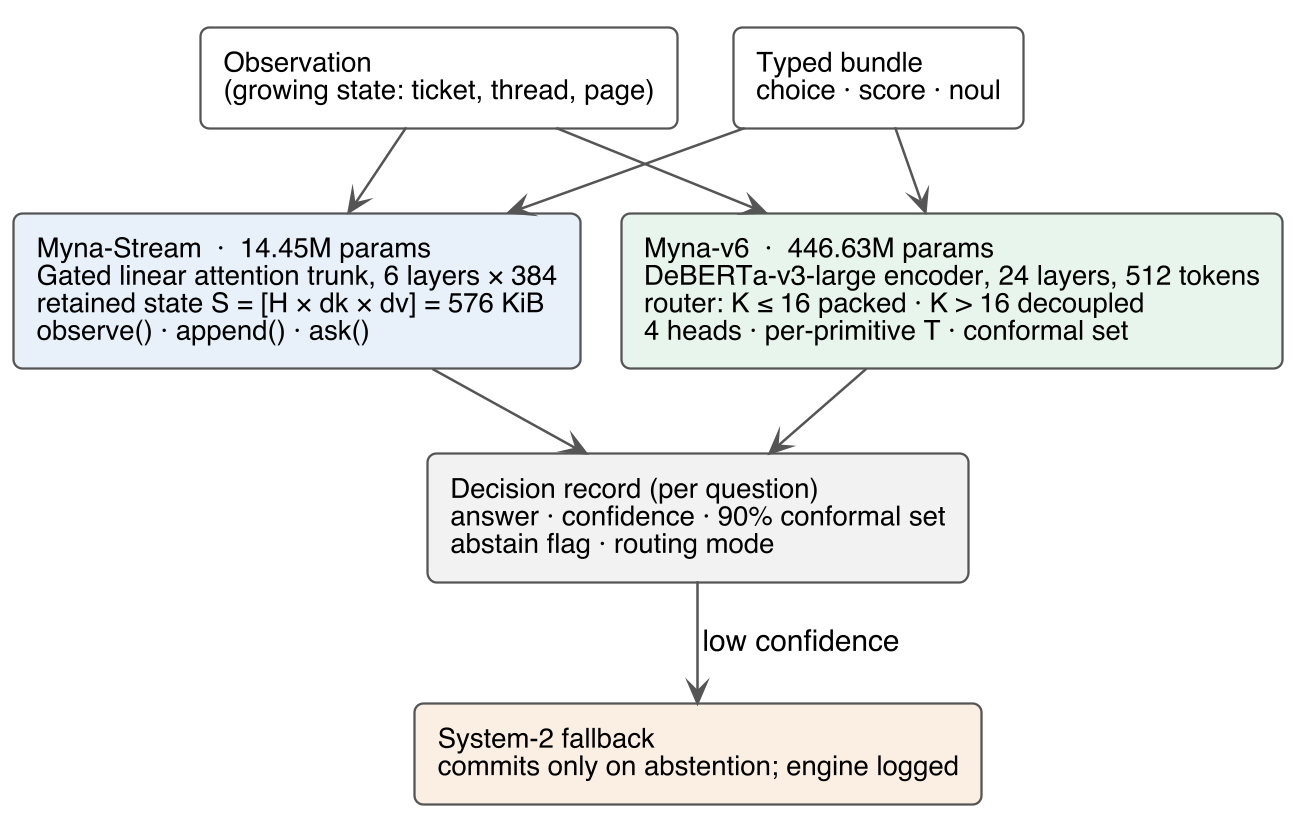
\includegraphics[width=0.9\linewidth]{paper/figures/fig1_architecture.png}
\caption{The two Myna{} engines behind one typed contract. Myna-Stream{} scans a growing observation
once into a 576 KiB state and answers from the cache; Myna-v6{} re-encodes the state on every
question and routes by option cardinality. Both write the same decision record, and a
low-confidence answer can be deferred to a second engine with the committing engine logged. The
figure is a schematic; the measurements are in Section~8.}
\end{figure}

\begin{table}[t]
\centering
\footnotesize
\caption{The frozen \textsc{decision-v2-pilot} suite (11 public sources). Cells are the 16
$(\text{source},\text{question})$ pairs; $K$ is the number of options per question.}
\begin{tabular}{lrrrr}
\toprule
Split & Rows & Questions & Cells & $K$ \\
\midrule
Train & 57{,}904 & 73{,}804 & 16 & 2--77 \\
Development & 1{,}176 & 1{,}440 & 16 & 2--78 \\
Calibration & 448 & 568 & 16 & 2--77 \\
Test & 1{,}176 & 1{,}440 & 16 & 2--78 \\
\bottomrule
\end{tabular}
\end{table}

\section*{4. Cardinality Is a Budget}
\subsection{The packed layout and its failure}
The packed scorer spends one sequence on the prefix, the state, and all option spans. Each span is
the option text, one \texttt{[MASK]}, and a separator. The state is truncated first, and if the
option spans still exceed the window, the fallback keeps a prefix of the options and collapses
the context to a single token. That fallback is not a graceful degradation: it deletes the state
and the tail options at the same time.

The budget was measured on every test cell with the suite's own renderer and tokenizer
(Figure~2). The 15 non-banking77 cells have $K=2$--$15$; none overflows, and
every option receives a mask. The 77-way banking77 cell differs: mean option-span length is 490.3
tokens, or 6.36 tokens per option; with a median 25-token state, the total exceeds 512 on 50 of
116 rows. Across the cell the fallback keeps a mean of 75.9 options and drops up to 6, and on
overflow rows it also reduces the context to one token. The collapse is a budget failure, not a
tokenization artifact.

\subsection{An isolated routing ablation}
The router sends $K\le16$ to the packed scorer and $K>16$ to the set-aware head. The threshold is
a design cap, not a measured optimum: every cell at or below 15 options fits with zero drops, and
the only cell above the cap is the 77-way one. Sixteen leaves one option of headroom.

Because the earlier campaign changed both the router and the model between arms, the routing
effect was re-measured on one checkpoint. The packed scorer was forced on every cell with
\texttt{-{}-max-packed 1000}, and the same weights were then scored with the router enabled.
Table~2 reports the result. Forcing the packed path scores 0.0345 on banking77
and 0.7378 macro; routing scores 0.6724 and 0.7777. The difference is $0.6379/16=0.0399$ macro,
and the other 15 cells are identical to the last digit, because the same weights take the same
path on them. This is a budget repair for exactly one cell.

\begin{table}
\centering
\footnotesize
\caption{The routing ablation on one checkpoint, same weights, same rows, same decoding. Only the
packed/decoupled switch changes. Every cell except banking77 is identical, so the macro difference
is one cell divided by sixteen.}\begin{tabular}{lrrr}
\toprule
Arm & banking77 ($n=116$) & other 15 cells & 16-cell macro \\
\midrule
packed everywhere (\texttt{-{}-max-packed 1000}) & 0.0345 & 0.7847 & 0.7378 \\
routed ($K>16$ decoupled) & 0.6724 & 0.7847 & 0.7777 \\
\midrule
difference & $+0.6379$ & $0.0000$ & $+0.0399$ \\
\bottomrule
\end{tabular}
\end{table}

\subsection{The cost of routing}
Routing is not free. Under the packed path a question is one sequence; under the decoupled path it
is $K$ sequences, one per option. On the 77-way cell the decoupled path therefore runs 77 encoder
passes where the packed path runs one, and the measured cost follows: over six banking77
questions in one warm process, the median call is 4.90 s under the decoupled path and 0.43 s
under the packed path, a ratio of 11.4. The router buys accuracy on that cell at that price, and it is only
correct to pay it when the packed path has already failed. A deployment that routes on
cardinality alone pays it on every high-cardinality question, including ones the packed path
could have answered.

\subsection{What routing does not buy}
Routing is not a general accuracy method. The improvement is confined to the single cell whose
option spans do not fit, the other 15 cells are unchanged, and the representation is unchanged.
The result is a budget-allocation finding, not an architectural contribution, and it does not
support a broad accuracy claim.

\begin{figure}
\centering
\includegraphics[width=0.9\linewidth]{paper/figures/fig2_cardinality.pdf}
\caption{(a) The packed window is a budget: each point is a cell's median state plus option-span
tokens at its maximum $K$; the 77-way cell sits on the 512-token line. (b) The isolated routing
ablation: on one checkpoint, forcing the packed path scores 0.0345 on banking77 and enabling the
router scores 0.6724, with the other 15 cells identical.}\end{figure}

\section*{5. External Baselines and Comparison Footing}
\subsection{The comparison set}
Table~3 places the Myna{} arms beside five external references on the same 1{,}176
test bundles. Two are contemporary decision engines evaluated by their own released harnesses:
Laya 0.4.19, in three configurations, and VegaML 0.15.0. Three are classical references: a
train-prior majority classifier, a supervised TF-IDF unigram/bigram classifier with logistic
regression, and a zero-shot NLI scorer (\texttt{cross-encoder/nli-deberta-v3-small}).

The footing differs by arm, and the difference is large enough that it must travel with the
numbers. Myna-v6{} is fine-tuned on the suite's train split and is therefore in-domain on all 16
cells. The classical references are trained on the same split, so they are in-domain too, but
they are given only the state text and the question instructions, not the option descriptions.
Laya and VegaML are evaluated zero-shot: Laya's training mixture covers 6 of the 16 cells (the
five agnews cells and boolq), and VegaML is out-of-domain on all 16. The comparison is therefore
an in-domain fine-tuned encoder against two out-of-domain engines and three classical supervised
references, and no single column is a like-for-like statement about model quality.

\subsection{What the table shows}
Myna-v6{} reaches 0.7777 macro, 0.7882 overall, and 0.7509 joint bundle exact. The strongest
external reference is the supervised TF-IDF classifier at 0.7111 macro, 0.6840 overall, and
0.6293 bundle exact, followed by the best Laya configuration at 0.7050, 0.6792, and 0.6182.
VegaML 0.15.0 reaches 0.6160, the majority classifier 0.3726, and the zero-shot NLI scorer 0.3278.
The row-clustered 95\% interval on the Myna-v6{} macro is [0.7601, 0.7946]; the interval on joint
bundle exact is [0.7318, 0.7696]. The baselines' per-question records are not released in a form
that supports a paired interval, so their columns are point estimates.

The aggregate hides three losses that matter for the interpretation. On the three ordinal cells
(amazon/stars, sst5/sentiment, yelp/rating) the TF-IDF classifier scores 0.5250, 0.3750, and
0.4375 while Myna-v6{} scores 0.1750, 0.1500, and 0.2000. On agnews/is\_business and
agnews/is\_scitech, Laya scores 0.8837 and 0.9388 against 0.9535 and 0.9184. The aggregate lead
is therefore carried by the choice and boolean cells, not by the ordinal primitive, and
Section~10 shows that the ordinal primitive is at chance.

\begin{table}
\centering
\footnotesize
\caption{All arms on the same 1{,}176 bundles and 1{,}440 questions. Macro is the unweighted mean
over the 16 cells; bundle exact is the fraction of bundles in which every question is correct.
Laya is in-domain on 6 of 16 cells and zero-shot on 10; VegaML is zero-shot on all 16; Myna-v6{} is
in-domain on all 16. The two Myna{} rows differ only in the routing switch.}
\begin{tabular}{lrrrr}
\toprule
Arm & macro & overall & bundle & footing \\
\midrule
Myna v6, routed & \textbf{0.7777} & 0.7882 & 0.7509 & in-domain \\
Myna v6, packed everywhere & 0.7378 & 0.7368 & 0.6879 & in-domain \\
TF-IDF + logistic regression & 0.7111 & 0.6840 & 0.6293 & in-domain, text only \\
Laya 0.4.19 (typed-decisions best) & 0.7050 & 0.6792 & 0.6182 & 6/16 in-domain \\
Laya 0.4.19 (raised + tournament) & 0.6829 & 0.6597 & 0.5918 & 6/16 in-domain \\
Laya 0.4.19 (English default) & 0.6624 & 0.6333 & 0.5595 & 6/16 in-domain \\
VegaML 0.15.0 & 0.6160 & 0.5833 & 0.5119 & zero-shot \\
Train-prior majority & 0.3726 & 0.2965 & 0.2041 & in-domain \\
Zero-shot NLI & 0.3278 & 0.3465 & 0.3027 & zero-shot \\
\bottomrule
\end{tabular}
\end{table}

\begin{figure}
\centering
\includegraphics[width=0.9\linewidth]{paper/figures/fig3_external.pdf}
\caption{All nine arms on the same 1{,}176 test bundles. Bars are 16-cell macro; diamonds are
joint bundle exact. The ordering is stable under both aggregates. The Myna row is in-domain and
the two decision engines are out-of-domain or zero-shot on most cells, so the figure ranks
performance on this suite, not model quality in general.}
\end{figure}

\section*{6. Bundle Consistency: An Observed Property}
A bundle can contradict itself: an article can be labelled ``sports'' while the answer to ``is
this article about sports?'' is ``no''. The suite contains 172 bundles that ask both questions:
92 agnews bundles with a topic question and two of the four class booleans, and 80 yelp bundles
with a star rating and a recommendation question.

The checkpoint's summary records 0/172 contradictions. That record is reproducible: the rule that
produced it is in the campaign notebook's graph-ablation cell (\texttt{release/notebooks/}), and
re-implemented as code it gives 0/172 for Myna-v6{}, 1/172 for Laya, and 2/172 for VegaML. The rule
is narrow. It counts a bundle only when the bundle carries both a \texttt{choice} and a
\texttt{noul} question, the predicted option text appears inside the boolean question, and the
boolean is answered ``no''. It cannot see a yelp rating/recommendation contradiction, because the
rating is a \texttt{score} question, and it misses any pair whose option text is not a substring
of the question.

This paper therefore reports two numbers: the campaign rule, and a broader predicate that covers
both sources (\texttt{src/myna/consistency.py}; recomputed by
\texttt{bench/consistency\_audit.py}). A bundle is a contradiction under the broader predicate iff
the predicted topic is class $c$, the bundle asks \texttt{is}$\_c$, and the answer is ``no''; or
the predicted rating is 4--5 while \texttt{recommend} is ``no'', or 1--2 while \texttt{recommend}
is ``yes''. Under it, Myna-v6{} has 3 contradictions in 172 bundles, Laya has 31, and VegaML has 32
(Table~4). The Myna-v6{} rate is 1.7\%, and the three errors are two agnews
bundles and one yelp bundle.

This is a property of the fine-tuned encoder, not of the architecture. The checkpoint stores a
cross-question graph head whose gate is exactly zero in the v5 ablation (graph-on and graph-off
return identical predictions on both splits), the inference path never calls it, and no consistency
term was trained: the campaign config defines a consistency weight that no cell reads, and the
training loop minimizes per-question cross-entropy (\texttt{release/notebooks/}, cell 9). The paper
therefore makes no claim that the architecture enforces consistency, and it does not present the
measurement as a methodological contribution. It is a descriptive statistic
that a deployment can monitor, and it is the statistic on which Myna-v6{} has its largest margin
over the two external engines.

\begin{table}[t]
\centering
\footnotesize
\caption{Bundle consistency, same 172 bundles, under the campaign's recovered rule and under the
broader released predicate. The campaign column re-implements the notebook rule and reproduces the
published 0/172 for Myna; the released column also counts the yelp rating/recommendation pair that
the campaign rule cannot see.}\begin{tabular}{lrrrr}
\toprule
Engine & campaign rule & released predicate & agnews & yelp \\
\midrule
Myna v6 & 0/172 & 3/172 & 2 & 1 \\
Laya 0.4.19 & 1/172 & 31/172 & 5 & 26 \\
VegaML 0.15.0 & 2/172 & 32/172 & 26 & 6 \\
\bottomrule
\end{tabular}
\end{table}

\section*{7. Calibration, Selective Prediction, and Conformal Sets}
\subsection{Temperature scaling and calibration error}
The checkpoint stores three temperatures, 0.9 for \texttt{choice}, 0.9 for \texttt{score}, and
0.85 for \texttt{noul}, fitted per primitive by minimizing negative log-likelihood over a
temperature grid. They produce zero argmax flips between development and test, so the calibration
step changes probabilities but not decisions. The released notebook fits such a grid on the
development split and produces the v5 values (1.25, 1.0, 1.0); the cell that produced the v6
values is not among the released notebooks, so they are reported as stored in the checkpoint
rather than as reproduced. On the 1{,}440 test
questions the 10-bin expected calibration error is 0.0637 and the top-1 Brier score is 0.1187.
Figure~4a is the reliability diagram. The largest bin holds 847 questions at
mean confidence 0.980 and accuracy 0.968; the mid-confidence bins are sharply overconfident, with
the 0.6--0.7 bin at mean confidence 0.647 and accuracy 0.431.

These numbers are worse than the ones this paper reported before the correction in
Section~10, and the difference is almost entirely the ordinal cells: a model
that is confident and wrong on 240 questions has a larger calibration error than one that is
confident and right.

\subsection{Selective prediction}
Selective prediction is a curve, not a point. Ranking the 1{,}440 test questions by top
probability gives accuracies of 0.9750 at 50\% coverage, 0.9653 at 60\%, 0.9345 at 70\%, 0.8837
at 80\%, and 0.8318 at 90\%. The curve is monotone in the required direction: abstaining on the
least confident questions buys accuracy at every operating point measured. The v0 streaming arm,
on the same calibration split, reaches a maximum of 0.596 at 10.0\% coverage and fails the same
target; the confidence mechanism is a property of the Myna-v6{} arm, not of the architecture family.

\subsection{Conformal prediction: a negative result}
A split-conformal variant was fitted per primitive on the calibration split. On test, its 90\% sets
cover 85.49\% of questions (1{,}231/1{,}440) and its 95\% sets cover 93.68\% (1{,}349/1{,}440).
Both are below nominal, and the 90\% shortfall is 4.5 points.

Marginal coverage is licensed by exchangeability, and exchangeability is questionable here on
three counts. The calibration and test splits differ in source mix; the questions of a bundle
share a state and are therefore dependent; and the option cardinality ranges from 2 to 78 within
the same primitive. A single marginal number cannot locate the violation, and the paper does not
claim to; what it can say is that the nominal guarantee does not hold on this split, and that the
shortfall is large enough to matter for an abstention policy.

The paper therefore does not use conformal sets as a coverage guarantee or as the abstention
method. The selective results above use temperature-scaled confidence and the risk--coverage
curve, which is the standard instrument for this setting. The engine still exposes a 90\% set for
callers that want a ranking signal, but no coverage claim is attached to it, and a deployment that
needs a calibrated abstention threshold should fit it on its own traffic rather than inherit this
one.

\begin{table}
\centering
\footnotesize
\caption{Calibration and selective prediction on the 1{,}440 test questions, recomputed from the
released per-question records. The conformal rows are reported as a negative result: both levels
are below nominal.}
\begin{tabular}{lr}
\toprule
Metric & Value \\
\midrule
ECE (10 bins) & 0.0637 \\
Brier (top-1) & 0.1187 \\
selective accuracy @ 50\% coverage & 0.9750 \\
selective accuracy @ 60\% coverage & 0.9653 \\
selective accuracy @ 70\% coverage & 0.9345 \\
selective accuracy @ 80\% coverage & 0.8837 \\
selective accuracy @ 90\% coverage & 0.8318 \\
conformal 90\% empirical coverage & 0.8549 \\
conformal 95\% empirical coverage & 0.9368 \\
\bottomrule
\end{tabular}
\end{table}

\begin{figure}
\centering
\includegraphics[width=0.9\linewidth]{paper/figures/fig4_calibration.pdf}
\caption{(a) Reliability on the 1{,}440 test questions, 10 bins; marker area is bin count. (b)
Risk--coverage on the same ranking. (c) Nominal versus empirical conformal coverage: 85.49\% at
90\% and 93.68\% at 95\%.}
\end{figure}

\section*{8. Systems: Constant State and Deployment}
\subsection{Latency with a constant state}
On one Apple M5, in one process, with the same state and question dictionary, Myna-Stream{} answers
33.08 ms at one question, 74.87 ms at five, 120.75 ms at ten, and 869.95 ms at fifty end-to-end.
With the state already cached, the ask-only path is 14.86 ms at one question, 55.45 ms at five,
98.22 ms at ten, and 787.12 ms at fifty. Ask is 10.1 ms fixed plus 9.6 ms per question with a
state slope of $-10.3$ $\mu$s/token, the fixed-size state measured; observe is 360 $\mu$s/token.
The ask-only path is the same engine with the scan removed, not a second model.

\subsection{MLX and the browser}
The same 14.45M checkpoint ports to MLX over identical weights, with no conversion step. MLX fp32
is 1.76--2.40$\times$ faster than PyTorch MPS from 128 to 16{,}384 state tokens; MLX int8 is
1.79--2.75$\times$ and 17.40 MiB on disk against 55.13 MiB. The ONNX export runs in Chrome 153
under WebAssembly at 59.32 MiB artifact, 73.09 MiB on the wire, a 394.4 ms cold load, and a 435.8
ms p50 for a three-decision session; all six parity checks pass, and the maximum probability drift
against the torch engine is $1.03\times10^{-6}$. The export's own parity check is
$8.94\times10^{-8}$ on the decision output.

\subsection{Why int8 is not deployed}
int8 is 3.17$\times$ smaller and not faster. Five of the six linear shapes this model uses are
slower quantized (0.43--1.06$\times$ fp32/int8) even though int8 reads 3.6$\times$ fewer weight
bytes, because the quantized pass gets 10--37 GB/s of weight read against fp32's 55--257 GB/s on
the same box. It is also not faithful: on 20 real questions the MLX int8 port moves option
probabilities by 9.24e-3 and flips one argmax on a question whose top two options were 0.0008
apart; the ONNX int8 artifact drifts 6.48e-2 and fails five browser checks. The fp32 path is deployed on
both routes, and the int8 artifacts remain in the tree for byte-constrained uses rather than for
speed.

\subsection{Two engines, one API}
The systems numbers are Myna-Stream{}'s, not Myna-v6{}'s. Myna-v6{} has no ONNX export and no browser
build, and it re-encodes the state, so a latency number for it would be a different experiment.
The shared API is what makes the split usable: an application can run Myna-Stream{} for high-frequency
decisions and defer to Myna-v6{} or another second-tier model on abstention, with the committing
engine logged. No end-to-end cascade accuracy is claimed, because no joint deferral policy was
trained.

\begin{table}
\centering
\footnotesize
\caption{Systems measurements on one Apple M5. Latency is p50, 10 repetitions, 3 warm-ups, same
process, same inputs. The MLX and browser rows are the 14.45M streaming arm, not Myna-v6{}.
``Cached'' is the ask-only path of the same engine.}
\begin{tabular}{ll}
\toprule
Metric & Value \\
\midrule
parameters & 14{,}449{,}280 \\
retained state & 576 KiB (589{,}824 B) at every length \\
end-to-end latency & 33.08 / 74.87 / 120.75 / 869.95 ms at 1 / 5 / 10 / 50 questions \\
ask-only latency & 14.86 / 55.45 / 98.22 / 787.12 ms at 1 / 5 / 10 / 50 questions \\
MLX fp32 vs MPS & 1.76--2.40$\times$; artifact 55.13 MiB \\
MLX int8 vs MPS & 1.79--2.75$\times$; artifact 17.40 MiB; 9.24e-3 drift, 1 argmax flip \\
ONNX browser & 59.32 MiB artifact, 394.4 ms cold, 435.8 ms p50, 1.03e-6 drift \\
ONNX int8 & 18.56 MiB; 6.48e-2 drift; 5 browser checks fail \\
\bottomrule
\end{tabular}
\end{table}

\begin{figure}
\centering
\includegraphics[width=0.9\linewidth]{paper/figures/fig5_systems_ours.pdf}
\caption{(a) p50 latency against the number of questions per request, same box and inputs; the
cached curve is the ask-only path of the same engine. (b) MLX fp32 and int8 against PyTorch MPS
over state lengths. (c) Artifact size; int8 is smaller but not faster and not faithful.}\end{figure}

\section*{9. What the Small Engine Does Not Do}
The streaming arm is a deployment result, not an accuracy result. Three measurements make that
concrete.

\textbf{Synthetic success does not transfer.}
The v0 checkpoint scores 0.9525 on the synthetic typed-decision test split, against a gate
threshold of 0.94. The v1b checkpoint, trained on the real suite, scores 0.3423 on the same
synthetic rows, which is below the 0.3546 majority floor; on the real suite it scores 0.4893
against a 0.4331 majority floor, and the data-path variant scores 0.5339. The synthetic task is
solved and the real 16-cell task is not.

\textbf{Removing the shortcut does not add the ability.}
A dose-matched anti-prior arm removes the majority-label shortcut: constant-emitter cells go from 4
to 0, blank-instruction accuracy rises from 0.3341 to 0.4315, and blank-options accuracy from
0.2669 to 0.3674. The same change drops test macro from 0.5339 to 0.4785. The mechanism moved as
designed and the accuracy moved down. Two caveats travel with the pair: the \emph{off} arm stopped
at step 3{,}314 of 3{,}600 and its harness prints VOID, and the \emph{on} arm is a continuation
rather than an uninterrupted run. The pair is a mechanism check, not a clean causal estimate.

\textbf{Long context is flat at chance.}
The 4k truncated-backprop arm scores 0.1833 at 4{,}096 state tokens and 0.1500 at 16{,}384; the
128-token rung is also 0.1500, against a 0.167 uniform floor. The harness prints
\texttt{readable: false} because the shortest rung is at chance: this is not a decay curve but a
model that never learned the task at any length. Steps 799 and 1199 agree exactly on all three
shared rungs, so the limiter is the mechanism rather than the dose.

\begin{table}
\centering
\footnotesize
\caption{The small-engine diagnostics. Synthetic and real columns are different suites: 0.9525 is
the synthetic test split; 0.4893--0.5339 are the real 16-cell suite. The anti-prior \emph{off} arm
stopped at step 3{,}314 of 3{,}600 and its harness prints VOID.}
\begin{tabular}{llrr}
\toprule
Arm & Data & macro & note \\
\midrule
v0 & synthetic & 0.9525 & gate 0.94 \\
v1b & synthetic & 0.3423 & below floor \\
v1b & real suite & 0.4893 & floor 0.4331 \\
anti-prior off & real suite & 0.5339 & 4 emitters; VOID \\
anti-prior on & real suite & 0.4785 & 0 emitters \\
v6 & real suite & 0.7777 & in-domain \\
lc1-4k, 4k state & needle & 0.1833 & readable:false \\
lc1-4k, 16k state & needle & 0.1500 & readable:false \\
\bottomrule
\end{tabular}
\end{table}

\section*{10. A Measurement Correction}
The revision of this paper uncovered a scoring error in the evaluation harness, and the corrected
numbers replace every earlier figure. The error is reported here rather than silently repaired,
because its signature is instructive and because the headline aggregates depend on it.

\textbf{The error.}
The suite stores an ordinal answer as a 1-based star level, while the option vector the model
scores is 0-based. The harness compared the two directly, \texttt{hit = top == ranked[gold]}, so a
prediction was recorded as correct when it named the level above gold. The prediction was correct;
the bookkeeping was not.

\textbf{The signature.}
On the 240 \texttt{score} questions the pre-correction rate was 0.6250. Under the corrected
comparison it is 0.1750, which is the uniform floor for five options. The pre-correction rate was
exactly the frequency with which the predicted index equalled the gold level, which is the
signature of the off-by-one rather than of a working ordinal head. A direct inspection of one row
confirms the reading: on \texttt{yelp/test/2720}, with a gold label of three stars, the engine's
argmax is the ``3 stars: average'' option at $p=0.574$, and the pre-correction record marks the
answer wrong.

\textbf{The effect.}
Table~8 lists the quantities that change. Macro falls from 0.8620 to 0.7777,
overall accuracy from 0.8632 to 0.7882, and joint bundle exact from 0.8393 to 0.7509. ECE rises
from 0.0190 to 0.0637 and Brier from 0.0434 to 0.1187, because a model that is confidently wrong
on 240 questions is less well calibrated than the old number suggested. Selective accuracy at 60\%
coverage falls from 0.9873 to 0.9653. The ranking of systems is unchanged: Myna-v6{} still leads the
supervised TF-IDF baseline at 0.7111 and the best Laya configuration at 0.7050.

\begin{table}[t]
\centering
\footnotesize
\caption{Quantities affected by the ordinal scoring correction. The competitor columns are
unaffected: Laya and VegaML store prediction and gold in the same space, and their correctness
flags agree with their own records on all 240 score questions.}\begin{tabular}{lrr}
\toprule
Quantity & before & corrected \\
\midrule
16-cell macro & 0.8620 & 0.7777 \\
overall accuracy & 0.8632 & 0.7882 \\
joint bundle exact & 0.8393 & 0.7509 \\
ECE (10 bins) & 0.0190 & 0.0637 \\
Brier (top-1) & 0.0434 & 0.1187 \\
selective accuracy @ 60\% & 0.9873 & 0.9653 \\
score primitive & 0.6250 & 0.1750 \\
\bottomrule
\end{tabular}
\end{table}

\textbf{The repair and its guard.}
The harness now subtracts one for the ordinal cell and stores the 1-based level, so
\texttt{pred == gold} is correct without a second convention. The aggregation script recomputes
every aggregate from per-question records and refuses a record whose correctness flag disagrees
with its own prediction and gold, which is the check that would have caught the error on the first
run. The pre-correction witness is kept under a \texttt{predates-fix} suffix, and the corrected
script reproduces 0.7777 from it, which shows that the difference is arithmetic rather than a
re-run artifact. The full record is \texttt{paper/MEASUREMENT-CORRECTION.md}.

\section*{11. Discussion and Limitations}
\textbf{Scope and footing.}
This is a controlled study on one frozen suite. The reported intervals are sampling error over the
1{,}176 rows of the split, not a population over checkpoints or datasets. The accuracy arm is
fine-tuned on the suite's train split, so all 16 cells are in-domain, while the two external
engines are out-of-domain on at least 10 cells and the NLI scorer is zero-shot. The paper
therefore does not claim out-of-domain generalization or state-of-the-art superiority. A second
training seed, an out-of-domain cell set, and a paired harness for the external engines are the
three measurements that would most strengthen the claims, and none is in this draft.

\textbf{The ordinal primitive.}
The most important negative result is that the \texttt{score} primitive is at chance while the
other two primitives are strong. The paper does not establish the cause. Candidate explanations
are the ordinal head that the released configuration disables, the packed layout that puts five
near-identical option strings in one sequence, and the training objective, which treats the
ordinal cell as a five-way choice. A supervised TF-IDF classifier reaches 0.525 on amazon/stars,
so the information is present in the text and the failure is in the model or its head. Isolating
which is a single experiment with the CORAL head enabled, and it is left open.

\textbf{What could not be verified.}
The campaign notebooks are released (\texttt{release/notebooks/}): they contain the bundle loader,
the example builder, the graph head, the training loop, the evaluation, the development-split
temperature fit, and the per-option banking77 head training. They end at the v5 unified checkpoint.
The cell that assembled the v6 checkpoint, the cell that fitted its three temperatures, and the
2{,}000-bundle calibration split are not among them; the committed calibration split has 448 rows
and 568 questions. The banking77 \texttt{none\_absent} decomposition is 0/12 here against 7/12 in the
training record, while the cell aggregate matches at 78/116 against the recorded 77/116.
Myna-v6{}'s 512-token maximum also puts the long-context question out of its reach. These gaps are
reported rather than reconstructed.

\textbf{Data and code availability.}
The frozen suite, the checkpoint, the per-question records for every Myna{} arm, both consistency
predicates, the campaign notebooks, the reference training implementation, and every table and
figure generator are released with the paper. The reference trainer reproduces the architecture
and objective and writes a checkpoint the engine loads; the campaign notebook that produced the released checkpoint remains unavailable, and the paper does not claim to reproduce its exact
trajectory.

\textbf{Ethics.}
Typed decisions are used in routing, moderation, and triage. An abstention flag is not a safety
guarantee: the confidence scores are not certified, the suite is English and public, and the labels
carry their sources' biases. A deployment should log the committing engine and keep a human in the
loop for high-stakes cells. This study measured latency and bytes, not energy.

\section*{12. Conclusion}
This paper reported a measurement study of a typed decision engine on a frozen 16-cell suite,
against two contemporary decision engines and three classical baselines. The accuracy arm reaches
0.7777 macro, 0.7882 overall, and 0.7509 joint bundle exact; the strongest external reference, a
supervised TF-IDF classifier, reaches 0.7111 macro, and the best external decision engine reaches
0.7050. The lead is carried by the choice and boolean primitives: the ordinal primitive is at
chance, and a classical classifier beats the fine-tuned model on all three ordinal cells.

Three further results are negative. Cardinality routing is a budget repair worth 0.0399 macro on
exactly one cell, and it multiplies the encoder passes on that cell by the option count.
Cross-question consistency is an observed property of the encoder (3/172 against 31/172 and 32/172
for the external engines), not an enforced constraint; the graph head that would enforce it is not
called. Split-conformal sets cover 85.49\% at a 90\% target, so the paper reports calibration error
and risk--coverage instead.

The revision also corrected a scoring error that had inflated the macro from 0.7777 to 0.8620. The
corrected numbers replace every earlier figure, and the harness now refuses a record whose
correctness flag disagrees with its own prediction and gold. The paper contributes a measured
account of what this class of engine delivers, where it fails, and how the failure was found.



\section*{A. Reproduction and Artifact Map}
Every number in this paper is read from a committed JSON artifact or recomputed by a script in the
repository. The main commands are:

{\scriptsize
\begin{verbatim}
python -m bench.v6_audit --ckpt "myna-v5-prototype 2" --split test --every 1 \
  --out runs/paper_v6_audit.json --md runs/paper_v6_audit.md \
  --metrics runs/paper_v6_test.metrics.json \
  --rowout runs/paper_myna_v6_test.rowoutcomes.json
python -m bench.v6_audit --ckpt "myna-v5-prototype 2" --split test --every 1 \
  --max-packed 1000 --out runs/v6_packed_forced.json \
  --rowout runs/v6_packed_forced.rowoutcomes.json
python -m bench.paper_numbers --out runs/paper_numbers.json
python -m bench.consistency_audit --out runs/consistency_audit.json
python -m bench.paper_bootstrap --out runs/paper_bootstrap.json
python -m bench.routing_cost --out runs/routing_cost.json
python -m bench.prob_dump --split test --out runs/v6_prob_test.jsonl
python paper/make_figures_v2.py
\end{verbatim}
}

The routed re-score takes 953 s on CPU for all 1{,}176 bundles and writes all 1{,}440 question
outcomes; the packed-forced arm takes 540 s. \texttt{bench/paper\_numbers.py} recomputes macro,
overall accuracy, joint bundle exact, the per-cell table, per-primitive accuracy, ECE, Brier, and
the risk--coverage curve from those records, and refuses a record whose correctness flag disagrees
with its own prediction and gold. The row-clustered intervals use 20{,}000 bootstrap replicates with
seed 20261104 and resample rows, not questions, because the questions of a bundle share a state.

The witnesses are \texttt{runs/paper\_v6\_audit.json}, \texttt{runs/paper\_v6\_test.metrics.json},
\texttt{runs/paper\_myna\_v6\_test.rowoutcomes.json}, \texttt{runs/v6\_packed\_forced.*},
\texttt{runs/paper\_numbers.json}, \texttt{runs/paper\_bootstrap.json},
\texttt{runs/routing\_cost.json}, \texttt{runs/consistency\_audit.json},
\texttt{runs/paper\_cell\_intervals.json}, \texttt{runs/external\_\{majority,tfidf,nli\}.json},
\texttt{runs/laya\_0419\_test.rowoutcomes.json}, \texttt{runs/vegaml\_0150\_test.rowoutcomes.json},
\texttt{runs/latency\_matched.json}, \texttt{runs/bench\_mlx\_int8.json},
\texttt{runs/browser\_g3.json}, and the diagnostics under \texttt{runs/g6\_*} and
\texttt{runs/needle\_*}.

\paragraph{The scoring correction.}
The pre-correction row outcomes are kept as
\texttt{runs/paper\_myna\_v6\_test.predates-fix.rowoutcomes.json}. The corrected aggregation script
reproduces 0.7777 macro from that file, which establishes that the change in
Section~10 is arithmetic and not a re-run artifact. The full record, including the
before-and-after per-cell table, is \texttt{paper/MEASUREMENT-CORRECTION.md}.

\paragraph{Known gaps.}
The campaign notebooks are in \texttt{release/notebooks/} with their digests and the cell ranges
that differ between the three copies. They cover the v5 training loop, the development-split
temperature fit, the per-option banking77 head, and the v5 checkpoint merge; they do not contain
the v6 assembly cell, the fit that produced the v6 temperatures, or the 2{,}000-bundle calibration
split. The calibration split committed here has 448 rows and 568 questions, and the 2{,}000-bundle
split in the model card is not committed and is not used for any number in this paper. The banking77 \texttt{none\_absent}
decomposition is 0/12 here against 7/12 in the training record while the cell aggregate matches at
78/116. These gaps are reported rather than reconstructed.

\section*{B. Per-Cell Results}
Table~9 reports the corrected per-cell re-score with row-clustered intervals.

\begin{table}
\centering
\footnotesize
\caption{Per-cell corrected re-score with row-clustered 95\% intervals (5{,}000 replicates, seed
20261104). The interval is on the cell accuracy; the unit resampled is the row, not the question.}
\begin{tabular}{lrrr}
\toprule
Cell & $n$ & Myna & 95\% CI \\
\midrule
agnews/is\_business & 43 & 0.9535 & [0.8837, 1.0000] \\
agnews/is\_scitech & 49 & 0.9184 & [0.8367, 0.9796] \\
agnews/is\_sports & 47 & 0.9787 & [0.9362, 1.0000] \\
agnews/is\_world & 45 & 1.0000 & [1.0000, 1.0000] \\
agnews/topic & 116 & 0.9052 & [0.8448, 0.9569] \\
amazon/stars & 80 & 0.1750 & [0.1000, 0.2625] \\
banking77/intent & 116 & 0.6724 & [0.5862, 0.7500] \\
boolq/answer & 80 & 0.8500 & [0.7750, 0.9250] \\
contrastive/decision & 196 & 0.9847 & [0.9643, 1.0000] \\
dbpedia14/category & 116 & 0.9569 & [0.9138, 0.9914] \\
imdb/positive & 80 & 0.9625 & [0.9125, 1.0000] \\
mnli/relation & 116 & 0.8621 & [0.8017, 0.9224] \\
sst5/sentiment & 80 & 0.1500 & [0.0750, 0.2375] \\
trec/answer\_type & 116 & 0.9483 & [0.9052, 0.9828] \\
yelp/rating & 80 & 0.2000 & [0.1247, 0.2875] \\
yelp/recommend & 80 & 0.9250 & [0.8625, 0.9750] \\
\bottomrule
\end{tabular}
\end{table}

The three ordinal cells are the only cells below 0.6, and they are the cells on which the corrected
harness changes the answer. The five agnews boolean cells and the contrastive cell are above 0.95.

\section*{C. Decision Sequence and Diagnostics}
Figure~6 gives the call sequence for one bundle. The readout is per question; no
cross-question constraint is applied. Figure~7 plots the small-engine
diagnostics of Section~9.

\begin{figure}
\centering
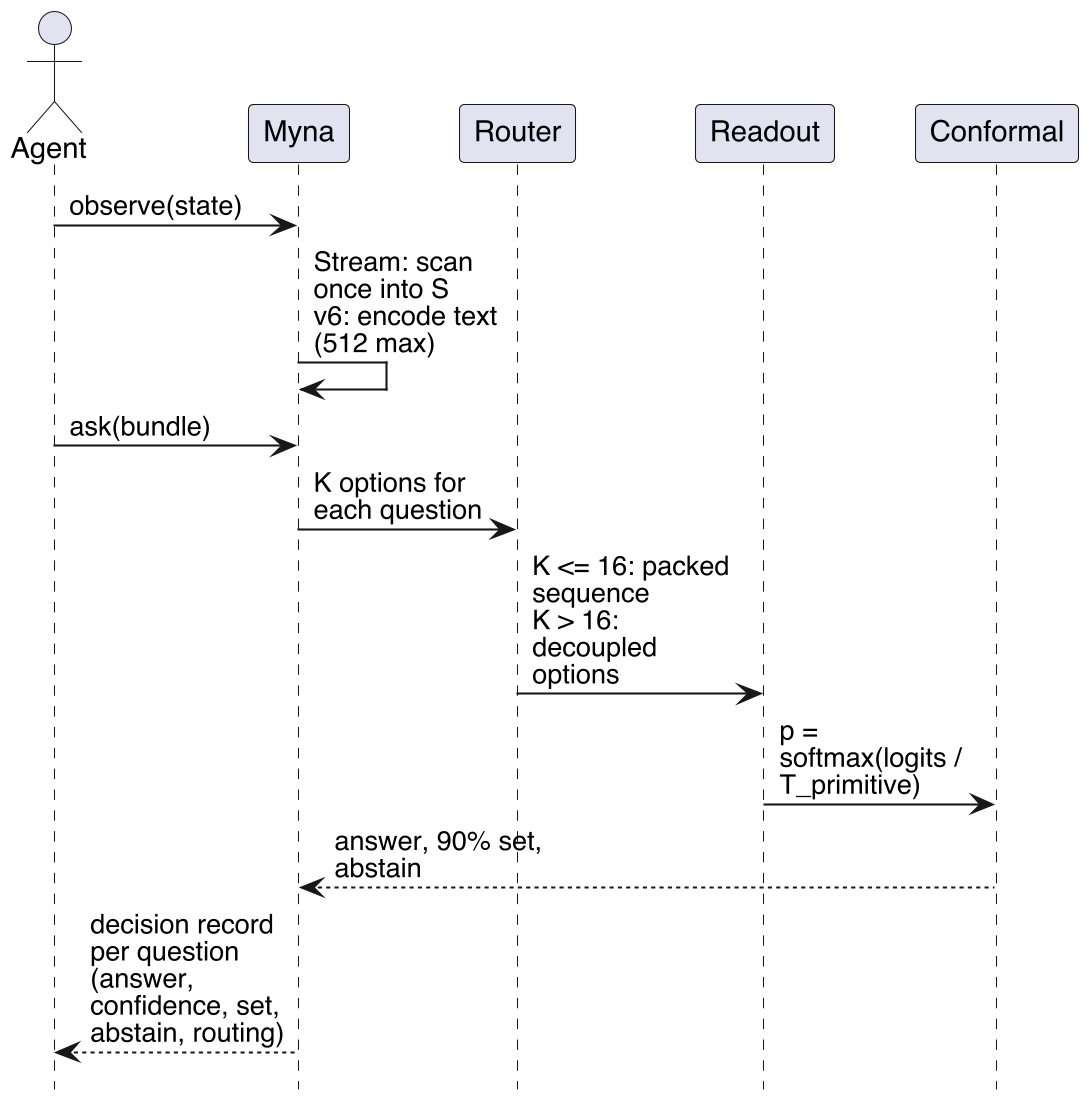
\includegraphics[width=0.9\linewidth]{paper/figures/fig7_sequence.png}
\caption{The Myna{} decision sequence for one bundle. The router chooses packed scoring for
$K\le16$ and decoupled scoring for $K>16$. The conformal gate can attach a 90\% set; this paper
does not use it as a coverage guarantee.}
\end{figure}

\begin{figure}
\centering
\includegraphics[width=0.9\linewidth]{paper/figures/fig6_diagnostics_journal.pdf}
\caption{(a) Synthetic versus real-suite macro. The dashed line is the 0.94 synthetic gate; the
dotted line is the 0.433 majority floor. The anti-prior arm removes four constant emitters and loses
0.0554 macro; the off arm is VOID. (b) Needle accuracy against state length for the 4k-trained arm:
flat at the 0.167 floor.}\end{figure}


\section*{References}

[1] Yinheng Li and Justin Wagle. LLM-as-Jev: LLMs Are Already Jev-Style Decision Models -- When and How to Fine-Tune Them. 2026.

[2] Feiyu Duan and Jiayu Lin and Jia Wang and Jun Xiang and Jialiang Wu and Xinnong Zhang and Hanqi Yan and Siyuan Wang and Zhongyu Wei. General Decision Models: Benchmarking and Insights Beyond Jev. 2026.

[3] Timo Schick and Hinrich Schütze. Exploiting Cloze Questions for Few Shot Text Classification and Natural Language Inference. Proceedings of the 16th Conference of the European Chapter of the Association for Computational Linguistics (EACL), 2021. doi:10.18653/v1/2021.eacl-main.20.

[4] Tianyu Gao and Adam Fisch and Danqi Chen. Making Pre-trained Language Models Better Few-shot Learners. Proceedings of the 59th Annual Meeting of the Association for Computational Linguistics (ACL-IJCNLP), 2021.

[5] Wenpeng Yin and Jamaal Hay and Dan Roth. Benchmarking Zero-shot Text Classification: Datasets, Evaluation and Entailment Approach. Proceedings of the 2019 Conference on Empirical Methods in Natural Language Processing (EMNLP-IJCNLP), 2019.

[6] Lewis Tunstall and Nils Reimers and Unso Eun Seo Jo and Luke Bates and Daniel Korat and Moshe Wasserblat and Oren Pereg. Efficient Few-Shot Learning Without Prompts. Proceedings of the 2022 Conference on Empirical Methods in Natural Language Processing (EMNLP), 2022.

[7] Angelos Katharopoulos and Apoorv Vyas and Nikolaos Pappas and François Fleuret. Transformers are RNNs: Fast Autoregressive Transformers with Linear Attention. Proceedings of the 37th International Conference on Machine Learning (ICML), 2020.

[8] Songlin Yang and Bailin Wang and Yikang Shen and Rameswar Panda and Yoon Kim. Gated Linear Attention Transformers with Hardware-Efficient Training. Proceedings of the 41st International Conference on Machine Learning (ICML), 2024.

[9] Albert Gu and Tri Dao. Mamba: Linear-Time Sequence Modeling with Selective State Spaces. Conference on Language Modeling (COLM), 2024.

[10] Bo Peng and Eric Alcaide and Quentin Anthony and Alon Albalak and Samuel Arcadinho and Stella Biderman and Huanqi Cao and Xin Cheng and Michael Chung and Matteo Grella and Kranthi Kiran GV and Xuzheng He and Haowen Hou and Jiaju Lin and Przemyslaw Kazienko and Jan Kocon and Jiaming Kong and Bartlomiej Koptyra and Hayden Lau and Krishna Sri Ipsit Mantri and Ferdinand Mom and Atsushi Saito and Guangyu Song and Xiangru Tang and Bolun Wang and Johan S. Wind and Stanislaw Wozniak and Ruichong Zhang and Zhenyuan Zhang and Qihang Zhao and Peng Zhou and Qinghua Zhou and Jian Zhu and Rui-Jie Zhu. RWKV: Reinventing RNNs for the Transformer Era. Findings of the Association for Computational Linguistics: ACL 2023, 2023.

[11] Tri Dao and Daniel Y. Fu and Stefano Ermon and Atri Rudra and Christopher Ré. FlashAttention: Fast and Memory-Efficient Exact Attention with IO-Awareness. Advances in Neural Information Processing Systems (NeurIPS), 2022.

[12] Iz Beltagy and Matthew E. Peters and Arman Cohan. Longformer: The Long-Document Transformer. Proceedings of the 58th Annual Meeting of the Association for Computational Linguistics (ACL), 2020.

[13] Chuan Guo and Geoff Pleiss and Yu Sun and Kilian Q. Weinberger. On Calibration of Modern Neural Networks. Proceedings of the 34th International Conference on Machine Learning (ICML), 2017.

[14] Yaniv Ovadia and Emily Fertig and Jie Ren and Zachary Nado and D Sculley and Sebastian Nowozin and Joshua V. Dillon and Balaji Lakshminarayanan and Jasper Snoek. Can You Trust Your Model's Uncertainty? Evaluating Predictive Uncertainty Under Dataset Shift. Advances in Neural Information Processing Systems (NeurIPS), 2019.

[15] Yonatan Geifman and Ran El-Yaniv. Selective Classification for Deep Neural Networks. Proceedings of the 34th International Conference on Machine Learning (ICML), 2017.

[16] Yonatan Geifman and Ran El-Yaniv. SelectiveNet: A Deep Neural Network with an Integrated Reject Option. Proceedings of the 36th International Conference on Machine Learning (ICML), 2019.

[17] Jing Lei and Max G'Sell and Alessandro Rinaldo and Ryan J. Tibshirani and Larry Wasserman. Distribution-Free Predictive Inference For Regression. Journal of the American Statistical Association, 2018. doi:10.1080/01621459.2017.1307116.

[18] Anastasios N. Angelopoulos and Stephen Bates. A Gentle Introduction to Conformal Prediction and Distribution-Free Uncertainty Quantification. 2021.

[19] Yaniv Romano and Evan Patterson and Emmanuel J. Candès. Conformalized Quantile Regression. Advances in Neural Information Processing Systems (NeurIPS), 2019.

[20] Surat Teerapittayanon and Bradley McDanel and H. T. Kung. BranchyNet: Fast Inference via Early Exiting from Deep Neural Networks. International Conference on Pattern Recognition (ICPR), 2016.

[21] Weijie Liu and Peng Zhou and Zhe Zhao and Zhiruo Wang and Haotang Deng and Qi Ju. FastBERT: a Self-distilling BERT with Adaptive Inference Time. Proceedings of the 58th Annual Meeting of the Association for Computational Linguistics (ACL), 2020.

[22] Ji Xin and Raphael Tang and Jaejun Lee and Yaoliang Yu and Jimmy Lin. DeeBERT: Dynamic Early Exiting for Accelerating BERT Inference. Proceedings of the 58th Annual Meeting of the Association for Computational Linguistics (ACL), 2020.

[23] Tim Dettmers and Mike Lewis and Younes Belkada and Luke Zettlemoyer. LLM.int8(): 8-bit Matrix Multiplication for Transformers at Scale. Advances in Neural Information Processing Systems (NeurIPS), 2022.

[24] Elias Frantar and Saleh Ashkboos and Torsten Hoefler and Dan Alistarh. GPTQ: Accurate Post-Training Quantization for Generative Pre-trained Transformers. International Conference on Learning Representations (ICLR), 2023.

[25] Guangxuan Xiao and Ji Lin and Mickael Seznec and Hao Wu and Julien Demouth and Song Han. SmoothQuant: Accurate and Efficient Post-Training Quantization for Large Language Models. Proceedings of the 40th International Conference on Machine Learning (ICML), 2023.
\end{document}
